\begin{description}
    \item[(1) Triangle inequality for the standard norm in $\R$:] 
\end{description}
$$\forall x,y \in \mathbb{R} ~~~~ |x+y| \leq |x| + |y|$$(more generally, $|x_1+...+x_n| \leq |x_1| + ... + |x_n| ~~~\forall x_1,...x_n \in \mathbb{R}$)

\begin{description}
    \item[(2) Reverse triangle inequality for the standard norm in $\mathbb{R}$: ] 
\end{description}
$$\forall x,y \in \mathbb{R} ~~~~\big| |x|-|y| \big| \leq |x+y|$$

\begin{description}
    \item[(3)] $\forall a,b \geq 0 ~ \forall \rho \geq 0$ $$ab \leq \frac{1}{2} \big(\rho a^2 + \frac{1}{\rho}b^2 \big)$$
    \begin{proof}
        \begin{align*} 0 \leq \big(\sqrt{\rho}a - \frac{1}{\sqrt{\rho}b} \big)^2 &= \rho a^2 + \frac{1}{\rho}b^2 - 2ab \\ &\implies2ab \leq \rho a^2 + \frac{1}{\rho}b^2 \\ &\implies ab \leq \frac{1}{2}\big(\rho a^2 + \frac{1}{\rho}b^2\big)\end{align*} \qed
    \end{proof}
\end{description}

\begin{description}
    \item[(4)]
    $\forall \overrightarrow{x} = \begin{bmatrix} x_1 \\ \vdots \\ x_n \end{bmatrix} \in \mathbb{R}^n ~~~ \forall \overrightarrow{y} = \begin{bmatrix} y_1 \\ \vdots \\ y_n \end{bmatrix} \in \mathbb{R}^n$ 
    $$|\overrightarrow{x} \cdot \overrightarrow{y}| \leq ||\overrightarrow{x}||_2\cdot||\overrightarrow{y}||_2$$
    That is, $$|x_1y_1+...+x_ny_n| \leq \big(\sqrt{x_1^2+...+x_n^2}\big)\big(\sqrt{y_1^2+...+y_n^2}\big) ~~~~ (*)$$
    \begin{proof}
    First, note that if $\overrightarrow{x} = \begin{bmatrix} 0 \\ \vdots \\ 0 \end{bmatrix}$, then $(*)$ holds. So we may assume $\overrightarrow{x} \not = \overrightarrow{0}.$ We have
    \begin{align*}
        |\overrightarrow{x} \cdot \overrightarrow{y}| &= \big| \sum \limits_{i=1}^nx_iy_i\big| \leq \sum \limits_{i=1}^n |x_iy_i| = \sum \limits_{i=1}^n|x_i|\cdot |y_i| \\ &\leq \sum \limits_{i=1}^n \frac{1}{2}\big(\rho |x_i|^2 + \frac{1}{\rho}|y_i|^2\big) \\ &=\frac{1}{2}\big[\rho ||{\overrightarrow{x}||_2}^2 + \frac{1}{\rho} {||\overrightarrow{y}||_2}^2\big]
    \end{align*}
    In particular, for $\rho= \frac{||\overrightarrow{y}||_2}{||\overrightarrow{x}||_2}$ we have 
    \begin{align*} |\overrightarrow{x} \cdot \overrightarrow{y}| = |\sum \limits_{i=1}^n |x_iy_i| &\leq \frac{1}{2} \big[\frac{||\overrightarrow{y}||_2}{||\overrightarrow{x}||_2} {||\overrightarrow{x}||_2}^2 + \frac{||\overrightarrow{x}||_2}{||\overrightarrow{y}||_2} {||\overrightarrow{y}||_2}^2\big] \\ &= \frac{1}{2} \big[||\overrightarrow{y}||_2 \cdot||\overrightarrow{x}||_2+||\overrightarrow{x}||_2 \cdot ||\overrightarrow{y}||_2\big] \\ &=||\overrightarrow{x}||_2 \cdot ||\overrightarrow{y}||_2 \end{align*} \qed
    \end{proof}
\end{description}

\begin{description}
    \item[(5)] Triangle inequality for $|| \cdot ||_2$ in $\mathbb{R}^n$:
    $$\forall \overrightarrow{x}=\begin{bmatrix}x_1\\ \vdots \\ x_n\end{bmatrix}, \overrightarrow{y}=\begin{bmatrix}y_1 \\ \vdots \\ y_n \end{bmatrix} \in \mathbb{R}^n, ~~~~ ||\overrightarrow{x} + \overrightarrow{y}||_2 \leq ||\overrightarrow{x}||_2 + ||\overrightarrow{y}||_2$$
    
    \begin{proof}
        \begin{align*}{||\overrightarrow{x} + \overrightarrow{y}||_2}^2 &= (\overrightarrow{x} + \overrightarrow{y}) \cdot (\overrightarrow{x} + \overrightarrow{y})  \\ &= \overrightarrow{x} \cdot \overrightarrow{x} + 2\overrightarrow{x} \cdot \overrightarrow{y} +\overrightarrow{y} \cdot \overrightarrow{y} \\ &= {||\overrightarrow{x}||_2}^2 + 2\overrightarrow{x} \cdot \overrightarrow{y} + {||\overrightarrow{y}||_2}^2 \\ &\leq {||\overrightarrow{x}||_2}^2 + 2{||\overrightarrow{x}||_2} \cdot {||\overrightarrow{y}||_2} + {||\overrightarrow{y}||_2}^2 &&(\text{Cauchy-Schwarz}) \\ &= \big({||\overrightarrow{x}||_2} + {||\overrightarrow{y}||_2} \big)^2 \end{align*}
        Hence,
        $${||\overrightarrow{x} + \overrightarrow{y}||_2}^2 \leq \big({||\overrightarrow{x}||_2} + {||\overrightarrow{y}||_2} \big)^2.$$Therefore, $$||\overrightarrow{x} + \overrightarrow{y}||_2 \leq {||\overrightarrow{x}||_2} + {||\overrightarrow{y}||_2}$$
        \qed
    \end{proof}
\end{description}

\begin{description}
    \item[(6)] Minkowski's Inequality: 
    $$\forall \overrightarrow{x}=\begin{bmatrix}x_1\\ \vdots \\ x_n\end{bmatrix}, \overrightarrow{y}=\begin{bmatrix}y_1 \\ \vdots \\ y_n \end{bmatrix} \in \mathbb{R}^n, ~~~~||\overrightarrow{x} + \overrightarrow{y}||_p \leq {||\overrightarrow{x}||_p} + {||\overrightarrow{y}||_p} ~~~~(p \geq1 \text{ a fixed number})$$ 
\end{description}

\begin{description}
    \item[(7)] Recall that $\forall a,b \in \mathbb{R} ~~\forall n \in \mathbb{N}$
    $$(a+b)^n= \sum \limits_{k=0}^n \binom nk a^kb^{n-k}$$
    So in particular, if $x \geq 0$ and $n \in \mathbb{N}$, then 
    \begin{align*} (x+1)^n &= \sum \limits_{k=0}^n \binom nk x^k 1^{n-k} \\ &=\sum \limits_{k=0}^n \binom nk x^k \\ &= \binom n0 x^0 + \binom n1 x^1 + ... + \binom nn x^n \\ &\geq1 + nx.
    \end{align*}
    Hence, $\forall x \geq 0 ~\forall n \in \mathbb{N} ~~~~(x+1)^n \geq 1 + nx.$
\end{description}

\begin{description}
    \item[(8) P-means: ] \leavevmode \\
    Let $x_1,...,x_n$ be positive real numbers. Let $p \in \mathbb{N} \cup {0}$. By the p-mean of $x_1, ..., x_n,$ denoted by $A_p(x_1, ..., x_n)$, we mean
    $$A_p(x_1, ..., x_n) = \begin{cases} \sqrt[p]{\frac{{x_1}^p+...+{x_n}^p }{n}} &p\not = 0 \\ \sqrt[n]{x_1+...x_n} &p=0 \end{cases}$$
    For example,
    \begin{align*}&p=1 &&A_1(x_1,...,x_n)=\frac{x_1+...+x_n}{n} &&&(\text{Arithmetic mean}) \\ &p=2 &&A_2(x_1, ..., x_n)= \sqrt{\frac{{x_1}^2+...+{x_n}^2}{n}} &&& \\ &p=0 && A_0(x_1,...,x_n) = \sqrt[n]{x_1+...x_n} &&& (\text{Geometric mean}) \end{align*}
    It can be shown that
    $$A_0(x_1+...x_n) \leq A_1(x_1,...,x_n) \leq A_2(x_1,...,x_n) \leq...$$
    In particular, $A_0 \leq A_1,$ that is 
    \begin{align*} &\sqrt[n]{x_1 + ... + x_n} \leq \frac{x_1+...+x_n}{n} &&(\text{AM-GM inequality}) \end{align*}
\end{description}

\begin{description}
    \item[(9) Jensen's Inequality:] Suppose $f:(a,b) \rightarrow \mathbb{R}$ is a convex function $\big(f''(x) \geq 0 \text{ for all } x \in (a,b)\big)$. Let $x_1,...,x_n$ be points $(a,b)$. Let $\lambda _1,... \lambda_n \geq 0$ such that $\lambda_1 +...+ \lambda_n = 1.$
    Then
    $$f(\lambda_1x_1 + ... + \lambda_nx_n) \leq \lambda_1f(x_1) +...+\lambda_nf(x_n)$$
    \item[Special Case: ]
    \begin{align*} &\begin{cases}&f(\lambda_1x_1 + \lambda_2x_2) \leq \lambda_1f(x_1) +\lambda_2f(x_2) \\ \\ &\lambda_1 + \lambda_2 = 1 \end{cases} \\ \\ &f\big((1-\lambda_2)x_1 + \lambda_2x_2\big) \leq \big(1-\lambda_2\big)f(x_1) +\lambda_2f(x_2) \end{align*}
\end{description}

\begin{figure}[h]
    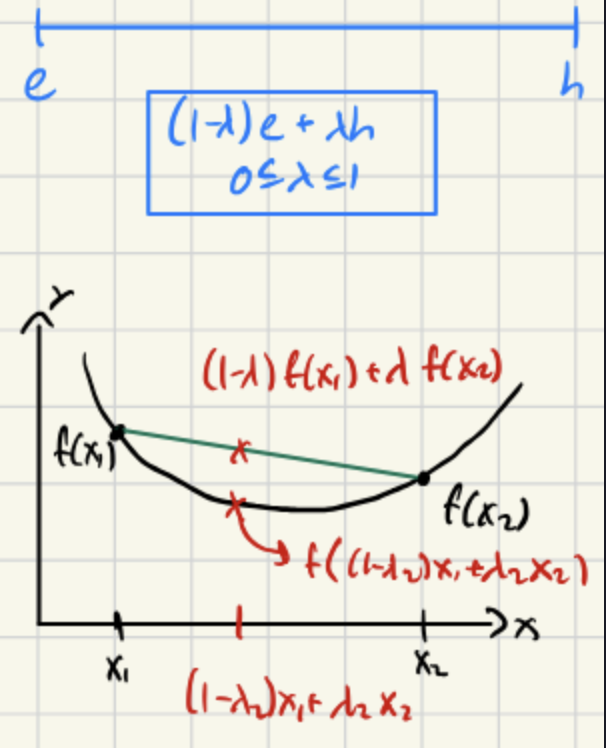
\includegraphics[width=.25\linewidth, center]{/Users/josiahvillarante/GradSchool/Grad-School-Notes/Math230A/Lecture/CH2/images/Jensen's Inequality.png}
\end{figure}